\newpage
\section{Gamification}
The gamification feature will be examined based on a framework to determine how well the implemented feature has achieved its intended purpose and its functionality. \\

The analysis includes four sections:\\
\begin{itemize}
    \item Functional Requirements - does the gamification feature fulfil the functional requirements set out in the project approach?
    \item Non-functional requirements - how well does the feature achieve the non functional requirements including performance and accessibility
    \item Scalability - how well does the feature perform with many topic groups, levels and users accessing the feature concurrently?
    \item Feedback from potential users of the feature - what do users such as lecturers, tutors and students think about the feature and how could it be improved?
\end{itemize}

\subsection{Functional requirements}

The functional requirements of the feature were analysed for completedness for both students, admins and backend.

\subsubsection{Requirements for Students}
7 out of 8 functional requirements for students have been completed.

\textbf{As a student, I need to be able to view all my enrolled topic groups and access weekly activities} - Incomplete requirement

The current implementation allows students to access the levels assigned to them through the topic groups they are enrolled in but it does not explicitly display the topic groups they are enrolled in on the gamification platform. The implementation of weekly activities was not completed as well due to time constraints.  This is a low priority requirement as it is an additional feature on top of the core functions of the platform. This would be classified under future work for the platform.

\newpage

\subsubsection{Requirements for Academics}
4 out of 6 functional requirements for academics have been fully completed with 1 functional requirement partially completed.

\textbf{As an Academic, I need to be able to create new timed questions of types (MCQ, True / False, Coding)} - Partially completed requirement

The question types of MCQ and True / False style questions have been implemented, however due to time constraints, the Coding type was not implemented. This was a decision made halfway through thesis C to omit this as it is a large complex piece of work but completion of other requirements was more important than this specific part of the requirement.

\textbf{As an Academic, I need to be able to customise the rewards awarded to students on completion of questions in modules. (Rewards Management)} - Incomplete requirement

Currently implemented is only points awarded on completion of a level. This requirement relates to badges and achievements that admins can customise for their own topic groups. This requirement was not completed due to time constraints and would similarly be classified as future work for the platform.

\subsubsection{Requirements for Backend}
8 out of 8 functional requirements for backend of gamification have been fully completed. All backend requirements support the frontend requirements and this was prioritised throughout the thesis to ensure that frontend requirements are able to be implemented.

\subsection {Non functional requirements}
\subsubsection {Performance and Accessibility}

There is room for improvement in terms of performance in the platform's current implemented state. There are no major performance issues that users will be able to observe but rather slighly longer page load times due to some heavy overheads of javascript that is being loaded on the platform. This is placing unecessary stress on the system that could be cleaned up as part of future works. Code clean up has been limited due to the time constraints and in hindsight, more time should have been allocated to refine and ensure code base is as clean as possible to decrease loading times.

The implemented platform scores well for accessibility due to the Chakra UI framework automatically adjusting to device size, allowing compatibility with screen readers and neatly tagging user interface elements approriately.

\begin{figure}[h!]
    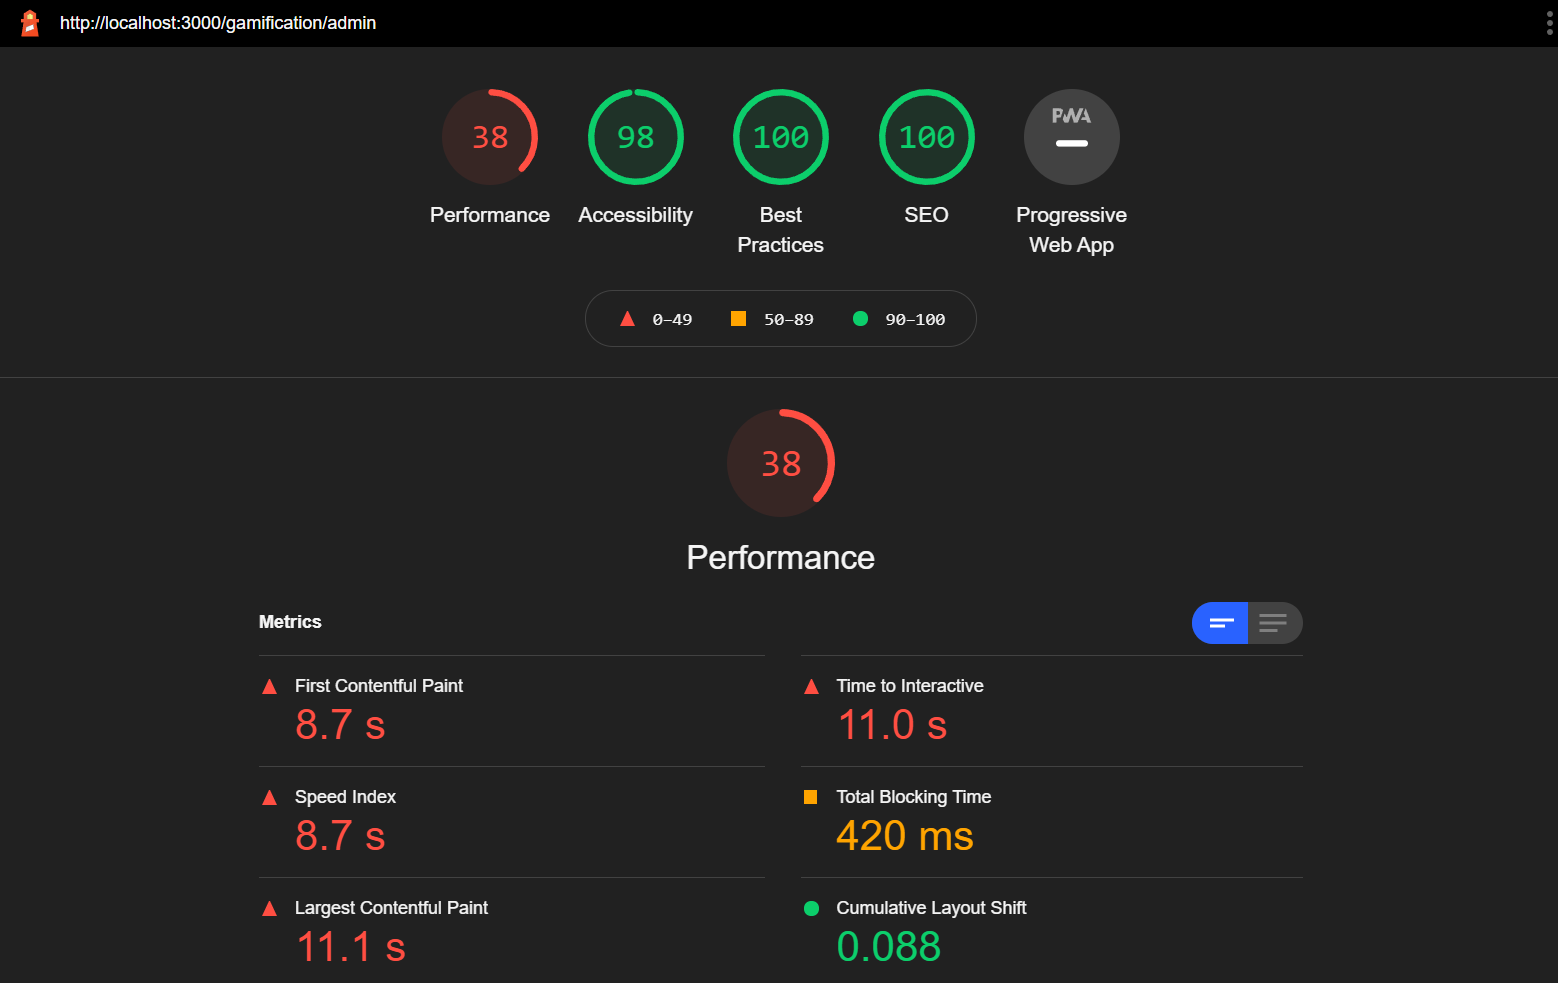
\includegraphics[scale=0.3]{gamification-accessibility}
    \centering
    \caption{Google Light House Report}
\end{figure}

\subsubsection{User Interface is easy to navigate}
The gamification platform pages have been based on the same core fundumentals of listing items in a grid list. This makes every page feel familiar for users and provide a consistent experience throughout. It also provides the flexibility in displaying different data objects using customised tiles throughout the platform. Overall this has been a great design choice and has helped to create a simple and easy to understand journey for both students and admins.

\subsubsection{Reusability}
User Interface design elements have been reused extensively. Examples include the grid list interface that is used across topic groups, levels, student dashboard, shop and repository. This decision has reduced the amount of development effort can is easily extendable to other use cases on the platform. The edit question and edit level pages are based on the same reused elements, simplifying and standardizing the look and feel for form submissions. Prompts and alerts are also reused to reduce development efforts. The repository page was designed to directly support reusabilty of levels across the whole platform by allowing admins to search for levels and add it into their own topic groups. Overall, the reusability score for the gamification platform is high and it has helped greatly in maximising the requirements implemented in the amount of time available.

\subsection{Scalability Testing}

The gamification platform scales well, the user interface are setup with grid lists which have no limits. This means that there is no limit on how many levels, topic groups or shop items on the platform. The only potential bottleneck could be the backend api server but that can be easily fixed through extra deployment of backend docker containers for load balancing. 

Similarly, if there was a bottleneck in the frontend when there are hundreds of users using the frontend concurrently, the platform can be scaled by increasing the number of docker containers and using nginx as load balancer to increase capacity. The features have been designed to support this form of scaling which is the industry standard. Each docker container can handle about 80 - 100 concurrent users and multiplying the number of docker containers will scale the platform up.

\subsection{Feedback from Potential Users}
\subsubsection{Students}

``The gamification platform has been an interesting take on learning modules, it is more exciting and the competitive aspect is really awesome!"

``The platform should limit how many times people can run through a level, that will increase competitiveness and sense of urgency."

Overall, across the students I have explained the platform to, the feedback has been positive, there are small details that they like to see to make it more robust and more competitive.

\subsubsection{Admins}

``It provides tutors more ways to test knowledge while encouraging students to actively do their best"

``This will definitely help to achieve learning outcomes especially in the online format."

Overall, across the tutors and lecturers I have explained the platform to, the feedback has been positive, they believed that this would add a way of learning and admin customisation that currently does not exist.

\newpage